\documentclass{beamer}
%\documentclass{powerdot}
%\documentclass{slides}[14pt]
%\pagestyle{empty}
%\normalsize
\usepackage{amsmath}
\usepackage{amssymb}
\usepackage{amscd}
% \usepackage{moreverb}
\usepackage{graphicx}
% \usepackage[all]{xy}
% \usepackage{beamerthemesplit}


\input macros			   %% loan from John Gibson's snowbird 07 talk
% \input ../../inputs/defsThesis     %% all Vaggelis edits: \renewcommand, etc

% Setup appearance:

\usetheme{Darmstadt}
\usefonttheme[onlylarge]{structurebold}
\setbeamerfont*{frametitle}{size=\normalsize,series=\bfseries}
\setbeamertemplate{navigation symbols}{}

% Standard packages

\usepackage[english]{babel}
\usepackage[latin1]{inputenc}
\usepackage{times}
\usepackage[T1]{fontenc}


% % Setup TikZ
% 
% \usepackage{tikz}
% \usetikzlibrary{arrows}
% \tikzstyle{block}=[draw opacity=0.7,line width=1.4cm]

\title{Recurrent spatio-temporal structures in presence of continuous symmetries}
\author{Evangelos Siminos}
\institute{Center for Nonlinear Science\\ School of Physics\\ Georgia Institute of Technology}
\date{March 23, 2009}

\begin{document}

\begin{frame}
  \titlepage
\end{frame}

\begin{frame}{Outline}
  \tableofcontents
\end{frame}

\section{Introduction}

\subsection{Dynamicist's vision of Turbulence}

\begin{frame}{Turbulence}
 	
\end{frame}

\begin{frame}{PO's and beyond}
\end{frame}

\subsection{This thesis}

\begin{frame}{Symmetry}
\end{frame}

\begin{frame}{\KSe}
 
\end{frame}

\section{(De-)symmetrization}

\subsection{$G$-background}
\frame{Isotropy}

\frame{Fixed point subspaces}

\subsection{Desymmetrization of \CLe}

\begin{frame}{\CLe}
  \begin{columns}[t]
    \column{.4\textwidth}
    \begin{exampleblock}{\CLe}
      	\[
		\begin{split}
			\dot{x} &=-\sigma x+ \sigma y \,,\\
			\dot{y} &=(r-z)x-a y \,,\\
			\dot{z} &= \frac{1}{2}\left(x y^*+x^*y\right)-b z\,.
		\end{split}
	\]
    \end{exampleblock}
     \begin{block}{ }
       $x,y\in\Clx{}$, $z\in\Rls{}$ parameters $\sigma,\,b\in\Rls{}$, $r=r_1+i\, r_2$, $a=1-i\, e$, $r_1,\,r_2,\,e\in\Rls{}$.
    \end{block}

    \column{.5\textwidth}
    \begin{exampleblock}{Equivariant under}
	$SO(2)$ acting by
      	\[
	\begin{split}
 		\Rot{\theta} (x,y,z) &= (e^{i\theta} x, e^{i\theta} y, z)\,, \\
			\theta	& \in[0,2\pi)\,.
	\end{split}
	\]
    \end{exampleblock}
    \begin{exampleblock}{Physics}
	For $r_2=0$ appears as a truncation of Maxwell-Bloch equation
	that describes ring laser with detuning proportional to $e$.
    \end{exampleblock}

  \end{columns}
\end{frame}

\begin{frame}
  \begin{columns}[t]
     \column{.6\textwidth}
	\begin{block}{}
	\begin{center}
		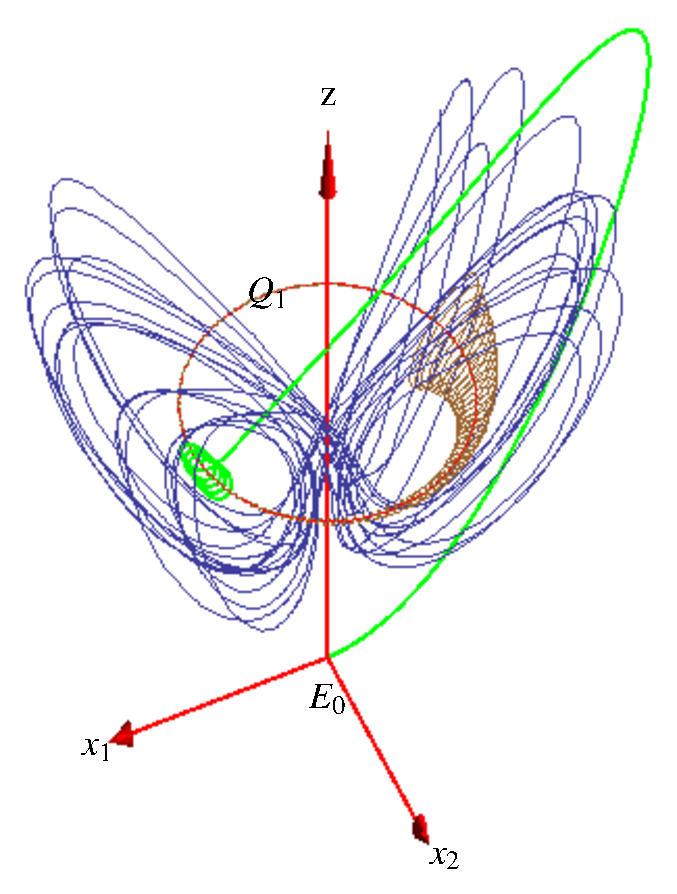
\includegraphics[width=.7\textwidth]{../../figs/CLE.eps}
	\end{center}
	\end{block}
     \column{.4\textwidth}
	\begin{block}{ }
	 ${r_1=28,}\, {b=8/3,}\,$ ${\sigma=10,}\, {a=1,}\,$ ${e=1/10,}\, {r_2=0}$
	\end{block}
	\begin{block}{ }
	  $E_0$: saddle\\
	  $Q_1$: relative equilibrium\\ 
	  $01$:  relative periodic orbit $T_{01}=1.542,\, \theta_{01}=2.953$
	\end{block}
   \end{columns}
\end{frame}






\section[\KSe]{\KS, $L=22$, phase space }

\subsection{\KSe}

\subsection{Antisymmetric subspace}

\subsection{Full space}

\section*{Summary}
\begin{frame}
\frametitle<presentation>{Summary}

In summary

\end{frame}


\end{document}
